\documentclass[floatfix,nofootinbib,superscriptaddress,fleqn]{revtex4-2}  
%\documentclass[aps,epsfig,tightlines,fleqn]{revtex4}
\usepackage[utf]{kotex}
\usepackage[HWP]{dhucs-interword}
\usepackage[dvips]{color}
\usepackage{graphicx}
\usepackage{bm}
%\usepackage{fancyhdr}
%\usepackage{dcolumn}
\usepackage{defcolor}
\usepackage{amsmath}
\usepackage{amsfonts}
\usepackage{amssymb}
\usepackage{amscd}
\usepackage{amsthm}
\usepackage[utf8]{inputenc}
 \usepackage{setspace}
%\pagestyle{fancy}

\begin{document}

\title{\Large 2022년 1학기 물리학 I: Quiz 15}
\author{김현철\footnote{Office: 5S-436D (면담시간 매주
    화요일-16:00$\sim$20:00)}} 
\email{hchkim@inha.ac.kr}
\affiliation{Hadron Theory Group, Department of Physics,
Inha University, Incheon 22212, Republic of Korea }
\date{Spring semester, 2022}


\vspace{1.cm}

\maketitle


\noindent {\bf 문제 1. (40 pt)} 
태풍이 불 때 어떤 집의 지붕 위에서 바람(공기의 밀도 1.20 $\mathrm{kg/m^3}$)의
속력은 100 km/h였다.
\begin{itemize}
\item[(가)] 지붕의 안과 밖의 압력차는 얼마인가? 
\item[(나)] 지붕의 면적이 100 $\mathrm{m^2}$일 때, 바람이 지붕을
  들어올리는 힘은 얼마인가? 
 \end{itemize}

 \noindent {\bf 풀이 : } 
 \begin{itemize}
  \item[(가)] 
  \item[(나)] 
 \end{itemize}




 \vspace{1.cm}

\noindent {\bf 문제 2. (60 pt)}
관의 지름이 $d$인 수도꼭지에서 물이 초기속도 $v$로 끊임없이 흘러나와서
아래로 떨어지고 있다(즉, 수도꼭지에서 나오는 물줄기의 지름이 $d$이고,
수도꼭지는 아래 방향을 향하고 있다). 수도꼭지에서 $h$만큼 떨어진 곳에서
물줄기의 지름은 얼마인가? 단, 공기의 저항은 무시하고, 물줄기는
끊어지거나 물방울이 되지 않는다고 가정한다.  
\begin{figure}[ht]
  \centering
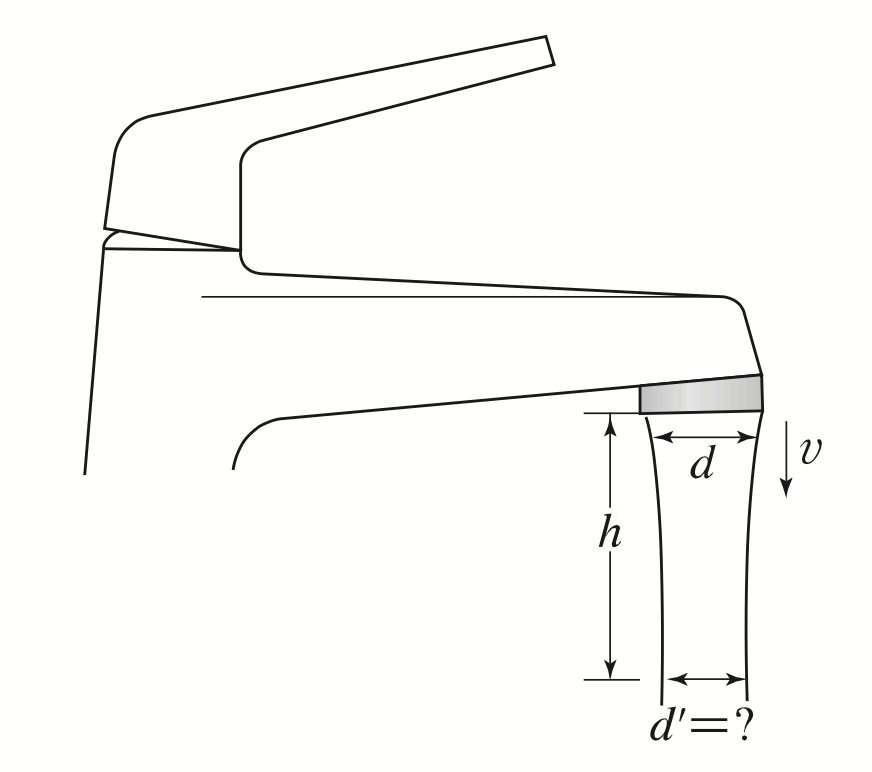
\includegraphics[scale=0.6]{Qfig17-1-20220509.png}
  \caption{문제 2}
  \label{fig:2}
\end{figure}

\noindent {\bf 풀이 : } 


\vspace{1.cm}
\noindent {\bf 문제 3. (50pt)  }
질량 0.500 kg인 물체가 가벼운 용수철(용수철 상수 $2.40\times 10^3$
N/m)에 매달려 마루 위에 있다. 
용수철을 평형지점에서 8.00 cm 압축하였다가 놓았을 때
\begin{itemize}
\item[(가)] 운동방정식을 세워라.
\item[(나)] 초기위상은 얼마인가?
\item[(다)] $t=0.25$ s일 때 물체의 위치를 구하여라.
\item[(라)] 이 계의 총 에너지를 구하여라.
\item[(마)] $x=+5.0$ cm와 $x=-5.0$ cm일 때의 속도를 각각 구하여라.
\item[(바)] 물체의 최대속도를 구하여라. 어느 지점에서 나타나는가?
 \end{itemize}

 \noindent {\bf 풀이 : } 
 \begin{itemize}
  \item[(가)] 
  \item[(나)] 
  \item[(다)] 
  \item[(라)] 
  \item[(마)] 
  \item[(바)] 
 \end{itemize}



 \vspace{1.cm}
\noindent {\bf 문제 4. (40pt)}
그림~\ref{fig:4}와 같이 반지름이 $R$이고 질량이 $M$인 원판, 링, 속이
꽉 찬 공,속이 텅빈 공을 길이가 $L$인 질량을 무시할 수 있는 실에 매달아
각 $\theta$까지 들어올렸다가 단진동을 시킨다. 
\begin{figure}[ht]
  \centering
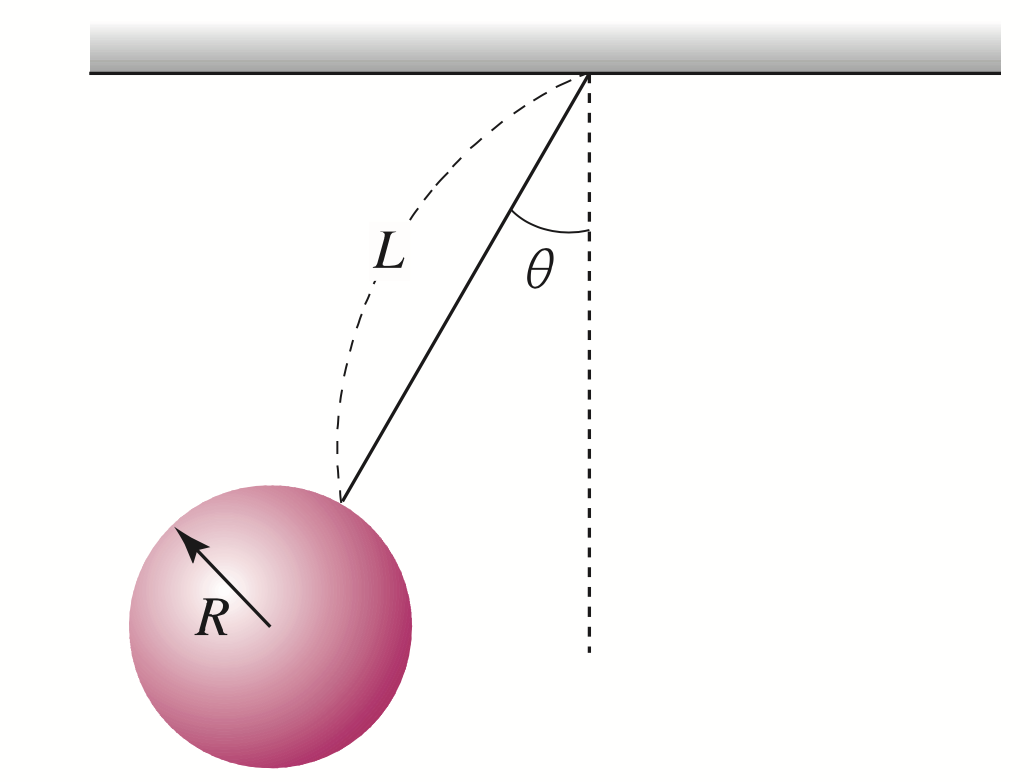
\includegraphics[scale=0.25]{Qfig17-4-20220509.png}
  \caption{문제 4}
  \label{fig:4}
\end{figure}
\begin{itemize}
\item[(가)] 단진동 주기가 가장 긴 것은 어느 것인가?
\item[(나)] 제일 아래 점에서 질량중심의 속력이 가장 큰 것은 어느 것인가?
\item[(다)] 이러한 진자를 달로 가져가서 똑같은 실험을 하면 주기는
  어떻게 되겠는가?
\item[(라)] 제일 아래 점에서 물체의 각속력을 $\omega$라 할 때 실의 장력은? 
\end{itemize}

\noindent {\bf 풀이 : } 
\begin{itemize}
  \item[(가)] 
  \item[(나)] 
  \item[(다)] 
  \item[(라)] 
\end{itemize}


\end{document}